\makeatletter
	\edef\cover@primarycolor{blue}
	\colorlet{cover@primarycolor}{\cover@primarycolor}
	\edef\cover@contourmargin{12.5mm}
	\edef\cover@trianglecorner{35mm}
	\edef\cover@techtrapeze{35mm}
	\edef\cover@textmargin{25mm}

\def\ddcoverpage{
	\noindent\begin{tikzpicture}[overlay, remember picture]
		% Draw background
		\fill[white!95!\cover@primarycolor] (current page.north west) rectangle (current page.south east);
		\node[anchor=north west, opacity=0.45] at (current page.north west)
			{
\includegraphics[height=\pageheight, keepaspectratio]{src/imgs/tile.jpg}};

		% Contour
		\coordinate			(contour-tl) at ([shift={(315:\cover@contourmargin)}] current page.north west);
		\coordinate			(contour-dr) at ([shift={(135:\cover@contourmargin)}] current page.south east);

		% Background image
		\coordinate			(bgimage-ul) at ([yshift=35mm] current page.south west);
		\coordinate			(bgimage-ur) at ([yshift=90mm] current page.south east);
		\begin{scope}
			\node[opacity=0, nosep, align=center] (imagebg) at ($(bgimage-ul)!0.5!(current page.south east)$)
				{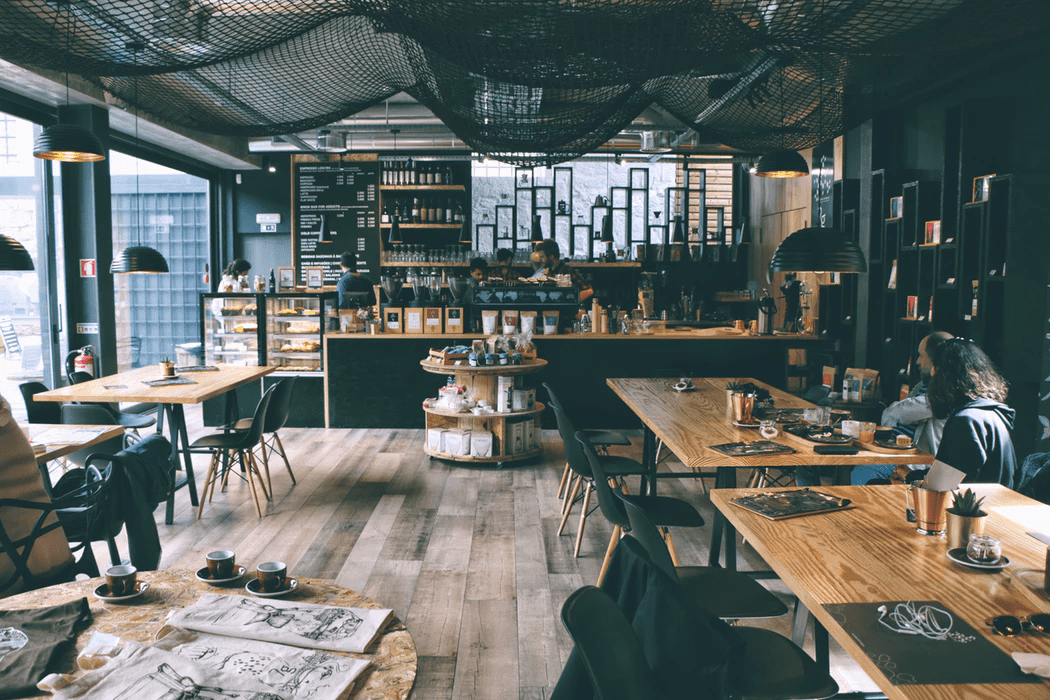
\includegraphics[keepaspectratio]{src/imgs/rest.png}};

			\clip (bgimage-ul)
			-- (bgimage-ur)
			-- (current page.south east)
			-- (current page.south west)
			-- cycle;

			\node[opacity=1.0, nosep, align=center] at (imagebg.center)
				{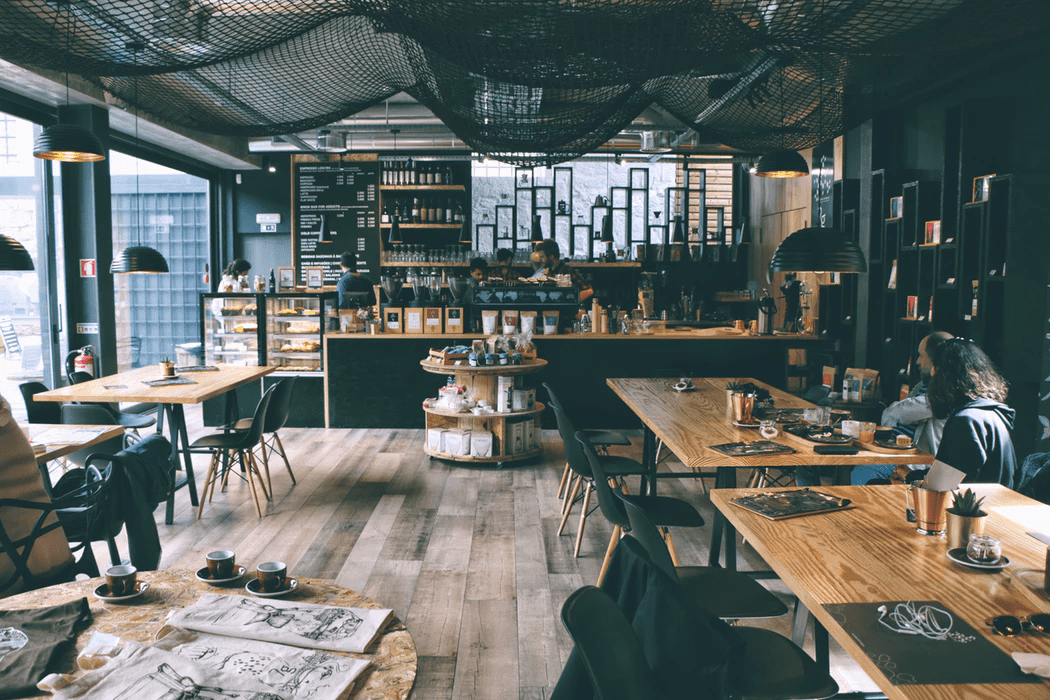
\includegraphics[keepaspectratio]{src/imgs/rest.png}};

			% Background overlay
			\fill[\cover@primarycolor!65!white, opacity=0.25] (bgimage-ul)
			-- (bgimage-ur)
			-- (current page.south east)
			-- (current page.south west)
			-- cycle;
		\end{scope}

		% Contour opacity
		\fill[opacity=0.3, white!20!cover@primarycolor] (contour-tl) rectangle (contour-dr);

		% Dot arounds
		\draw[cover@primarycolor!25!white, loosely dotted, line width=2pt, line join=round, line cap=round] (contour-tl)
		rectangle (contour-dr);

		% Upper left triangle
		\fill[cover@primarycolor] (current page.north west)
		-- ([yshift=-\cover@trianglecorner] current page.north west)
		-- ([xshift=\cover@trianglecorner] current page.north west)
		-- cycle;

		% Tech trape
		\fill[white] (bgimage-ul)
		-- ([yshift=\cover@techtrapeze] bgimage-ul)
		-- ([yshift=\cover@techtrapeze] bgimage-ur)
		-- (bgimage-ur)
		-- cycle;

		\fill[cover@primarycolor, opacity=0.45] (bgimage-ul)
		-- ([yshift=\cover@techtrapeze] bgimage-ul)
		-- ([yshift=\cover@techtrapeze] bgimage-ur)
		-- (bgimage-ur)
		-- cycle;

		% Techs
		\coordinate	(techtrape-center) at ($(bgimage-ul)!0.5!([yshift=\cover@techtrapeze] bgimage-ur)$);
		\node[imageset] (javaimg)			at (techtrape-center) {};
		\node[nosep, opacity=0.6] at ([shift={(195:2pt)}] javaimg) {\includeshadow[width=1.5cm, keepaspectratio]{src/imgs/java.png}};
		\node[nosep] at (javaimg) {
\includegraphics[width=1.5cm, keepaspectratio]{src/imgs/java.png}};
		\node[imageset] (reactimg)		at ([shift={(15:7cm)}] techtrape-center) {};
		\node[nosep, opacity=0.6] at ([shift={(195:2pt)}] reactimg) {\includeshadow[width=1.5cm, keepaspectratio]{src/imgs/react.png}};
		\node[nosep] at (reactimg) {
\includegraphics[width=1.5cm, keepaspectratio]{src/imgs/react.png}};
		\node[imageset] (postgreimg)	at ([shift={(195:7cm)}] techtrape-center) {};
		\node[nosep, opacity=0.6] at ([shift={(195:2pt)}] postgreimg) {\includeshadow[width=1.5cm, keepaspectratio]{src/imgs/postgresql.png}};
		\node[nosep] at (postgreimg) {
\includegraphics[width=1.5cm, keepaspectratio]{src/imgs/postgresql.png}};


		% Federico II logo
		\node[opacity=0.85] (fii-midpoint) at ([yshift=3.5cm] current page.south)
		{\color{white}
\includegraphics[width=4cm, keepaspectratio]{src/imgs/napoli_federico_ii.pdf}};

		% Fork Plate logo
		\coordinate (logo) at ($(current page.north)!0.33!(current page.south)$);
		\node[opacity=1] at ([shift={(215:8pt)}]logo)
		{\includeshadow[width=7cm, keepaspectratio]{src/imgs/fork-knife-plate.png}};
		\node[opacity=1] (logoimg) at (logo)
		{
\includegraphics[width=7cm, keepaspectratio]{src/imgs/fork-knife-plate.png}};

		% Details
		\coordinate (sidetext-bl) at ([xshift=5mm] contour-tl |- current page.west);
		\node [rotate=90] at (sidetext-bl)
		{\Lato\fontsize{8}{0}\selectfont Progetto di Ingegneria del Software, Università degli Studi di Napoli Federico II};

		% Title
		\node[nosep, anchor=south,text contour={[anchor=south]{1.75pt} at (logoimg.north){\fontsize{64}{0}\selectfont\AguafinaScript Ratatouille23}}] 
		(title-lbl) at (logoimg.north)
		{\color{cover@primarycolor!85!black}\fontsize{64}{0}\selectfont\AguafinaScript Ratatouille23};

		% Year
		\node[nosep, rotate=270, anchor=north west] (year-lbl) at ([shift={(215:4mm)}] contour-dr |- contour-tl)
		{\color{cover@primarycolor!30!black}\Gobold\fontsize{17}{0}\selectfont A.A. 2022-2023};

		% Authors
		\node[nosep, rotate=270, anchor=north west] (auth1) at ([yshift=-2pt] year-lbl.north east)
		{\color{cover@primarycolor!30!black}\Gobold\fontsize{9}{0}\selectfont amato ciro};
		\node[nosep, rotate=270, anchor=south west] (auth2) at ([yshift=-2pt] year-lbl.south east)
		{\color{cover@primarycolor!30!black}\Gobold\fontsize{9}{0}\selectfont vincenzo lombardi};

		% Group number
		\coordinate (gs-r) at (auth1.north east |- auth2.north east);
		\coordinate (gs-l) at (auth2.south east);
		\path[draw=cover@primarycolor!30!black, fill=cover@primarycolor!80!black] 
			([yshift=-5pt] gs-r)
			-- ([yshift=-8pt] gs-r)
			-- ([yshift=-8pt] gs-l)
			-- ([yshift=-5pt] gs-l)
			-- cycle;

		\node[nosep, opacity=0.75, rotate=270, anchor=west] (groupid) at ([yshift=-12pt] $(gs-r)!0.5!(gs-l)$)
			{\color{cover@primarycolor!30!black}\Gobold\fontsize{12}{0}\selectfont\ingswgroup};
	\end{tikzpicture}
	}
\makeatother

\begingroup\thispagestyle{empty}\null\ddcoverpage\newpage\tableofcontents\newpage\endgroup
